\RequirePackage{luatex85}
\documentclass[tikz, border=10pt]{standalone}

\usepackage[compat=1.1.0]{tikz-feynman}

\begin{document}
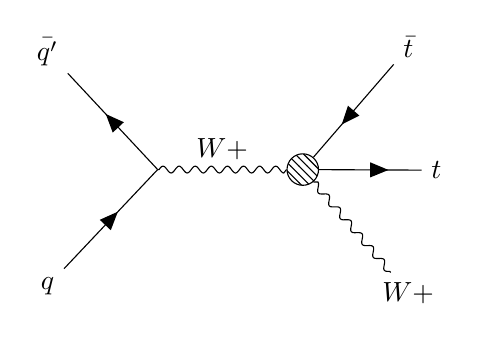
\begin{tikzpicture}
  \begin{feynman}
    \diagram [horizontal=a to b] {
      i1 [particle=\(q\)] -- [fermion] a -- [fermion] i2
      [particle=\(\bar{q'}\)],
      a -- [boson, edge label=\(W+\)] b [blob, minimum size=0.4cm],
      f1 [particle=\(W+\)] -- [boson] b,
      f2 [particle=\(t\)] -- [anti fermion] b -- [anti fermion] f3 [particle=\(\bar{t}\)],
      f1 -- [opacity=0] f2 -- [opacity=0] f3,
    };
  \end{feynman}
\end{tikzpicture}
\end{document}
